\documentclass{../tudscript}
\begin{document}
\begin{center}
\part*{Kern und Rang von Matrizen}
\end{center}
Ziel der Vorlesung:
\begin{flalign*}
A \cdot x = b \text{ lösbar} \iff \boxed{...}
\end{flalign*}
$a \in k^{m \times n}, x \in K^{1 \times n}, b \in K^{m \times 1}$
\sect{homogene LGS}
\begin{flalign*}
Ax = 0_{K^m}, \text{Lösungsmenge} L_h = \{x \in K^n | A \cdot x = 0_{K^m}\} \subseteq K^n
\end{flalign*}
$L_h$ ist ein Untervektorraum von $K^n$, denn:
\begin{enumerate}
\item $0_{K^{m \times n}} \in L_h$, denn $0_{K^n} \in K^n, A \cdot 0_{K^n} = 0_{K^m}$
\item $x_1 ,x_2 \in L_h$, denn: $x_1 + x_2 \in K^n, A(x_1, x_2) = Ax_1 + Ax_2 = 0 + 0 = 0 \Rightarrow x_1, x_2 \in L_h$
\item $x \in L_h, k \in K \Rightarrow kx \in L_h$, denn $kx \in K^n \land A(kx) = k \cdot Ax = k \cdot 0_{K^m} = 0$
\end{enumerate}
\ssect{Definition: Kern von Matrizen}
Sei $A \in K^{m \times n}$.
\begin{flalign*}
ker(A) := \{x \in K^{n} | Ax = 0_{K^n}\} \text{ heißt Kern von A}
\end{flalign*}
\paragraph{Bemerkung}
Der Kern einer Matrix A ist die Lösungsmenge des hom. LGS mit der Koeffizientenmatrix A.
\paragraph{Bemerkung}
Bemerkung: ker(A) ist ein UVR von $K^n$.

\ssect{Beispiel: Kern von Matrizen}
\begin{flalign*}
A = \begin{pmatrix}
1&1&1\\
1&-1&1\\
1&0&1
\end{pmatrix}_{3 \times 3}
%%%TODO
\rightsquigarrow ker(A) = \{t \ve{1}{0}{1} | t \in \bR\} 
\end{flalign*}
dim(ker(A)) = 1, 2 Zeilen in der Zeilenstufenform

\sect{inhomogene LGS}
\begin{flalign*}
Ax = b + 0_m, L = \{x \in K^m | Ax = b \} \subseteq K^n
\end{flalign*}
Bemerkung: L ist kein UVR von $K^n$, denn $0_k \notin L$

Bemerkung:
\begin{enumerate}
\item $x_1, x_2 \in L \Rightarrow X_2 - x_1 \in L_h$, denn
\begin{flalign*}
x_2 - x_1 \in K^n \land A(x_2 - x_1) = Ax_2 - Ax_2 = b - b = 0_{}K^n
\end{flalign*}
\item $x_1 \in L, x_2 \in L_h \Rightarrow x_1+x_2 \in L$, denn
\begin{flalign*}
x_1 + x_h \in K^n \land A(X_1 + x_h) = Ax_1 + Ax_h = b + 0 = b
\end{flalign*}
\end{enumerate}
\begin{enumerate}
\item $\underbrace{x_1}_{fest}, \underbrace{x_2}_{beliebig} \in L \Rightarrow X_2 - x_1 \in L_h		x_2 \in \underbrace{x_1 + L_h}_{\{x_1 + x_h | x_h \in L_h\}} bzw. L \subseteq x_1 + L_h$
\item sogar Gleichheit
\begin{flalign*}
x_1 \in L, x_h \in Lh \Rightarrow x_1 + x_h \in L \Rightarrow L \supseteq x_1 + L_h
\end{flalign*}
Bemerkung: 
\begin{flalign*}
\underbrace{L}_{\text{Lösungsmenge von Ax = b}} = \underbrace{x_1}_{\text{eine spezielle Lösung von Ax = b}} + \underbrace{L_h}_{Ax = 0}
\end{flalign*}
\end{enumerate}
\ssect{Beispiele}
\begin{flalign*}
A = \begin{pmatrix}
1&1&1\\
1&-1&1\\
1&0&1
\end{pmatrix}_{3 \times 3}
, b = \ve{3}{1}, \\
L = \{ \ve{1}{1}{1} + t \cdot \ve{1}{0}{-1} | r \in \bR \}
\end{flalign*}

\begin{flalign*}
L = \{ \ve{2+3s-4t}{s+2t}{-1-t} | s,t \in \bR \} \\
= \{ \ve{2}{0}{1} + s \ve{3}{1}{0} + t \ve{-4}{2}{-1} | s,t \in \bR \}
\end{flalign*}

$\ve{2}{0}{-1}$ ist eine spezielle Lösung des inh. Systems,\\
$L_h = Span(\{\ve{3}{1}{0}, \ve[{-4}{2}{-1}\})$

\ssect{Definition: affiner Teilraum}
Sei V ein K-VR, U ein UVR von V, $v \in V$.

\begin{flalign*}
v+U :=\{v+u | u \in U\} \textbf{\quad heißt affiner Teilraum von V}\\
dim(v+u) = dim U \textbf{\quad heißt Dimension des affinen Teilraums}
\end{flalign*}
Bemerkung: $v+U$ ist ein linearer Teilraum von V \\
$\iff \underbrace{v \in U}_{\text{andernfalls enthält v+U nicht den Nullvektor von V}}$
\ssect{Beispiele: affine Teilräume}
\begin{enumerate}
\item Lösungsmengen von inhomogenen LGS sind affine Teilräume (zugeordnet zum UVR des zugehörigen homogenen Systems)
\item Geraden, die parallel zu g sind stellen einen affinen Teilraum des UVR , der g bildet dar.
\begin{center}
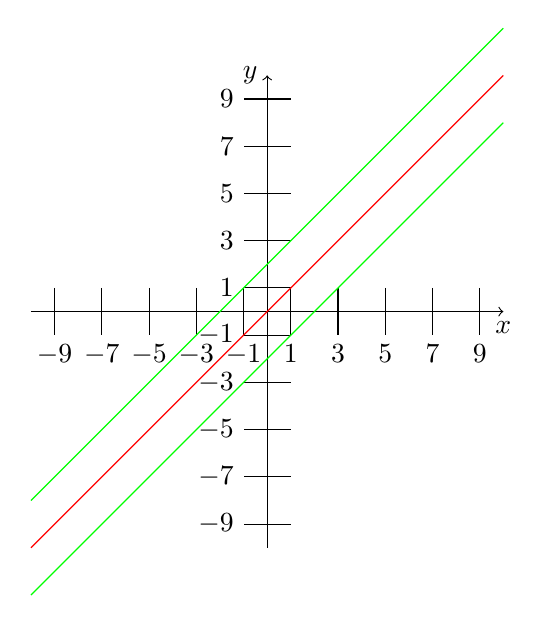
\begin{tikzpicture}[xscale=0.3,yscale=0.3,domain=-10:10,samples=800]
    \draw[->] (-10,0) -- (10,0) node[below] {$x$};
    \draw[->] (0,-10) -- (0,10) node[left] {$y$};
    \foreach \i in {-9,-7,...,9} {
        \draw (\i,1) -- (\i,-1) node[below] {$\i$};
    }
    \foreach \i in {-9,-7,...,9} {
        \draw (1,\i) -- (-1,\i) node[left] {$\i$};
    }
    \foreach \i in {2, -2} {
    	\draw[green] plot (\x,{\x+\i});
    }
    \draw[red] plot (\x,{\x});
\end{tikzpicture}
\end{center}


\end{enumerate}
Bemerkung: V K-VR,dim V = n

\begin{enumerate}
\item (0) heißen Punkte
\item (1) heißen Geraden
\item (2) heißen Ebenen
...
\item (n-1) Hyperebenen
\end{enumerate}
\sect{Lösbarkeitskriterium von LGS}
\begin{flalign*}
Ax = b		A = (s_1, s_2,..., s_n) \text{(s sind die Spaltenvektoren von A)}\\
Col(A) := Span(\{s_1, s_2, ..., s_n\}) \in K^m \\
\textbf{ heißt Spaltenraum von A (columns)}
\end{flalign*}
\begin{flalign*}
Col(A) = \{k_1 s_1 + ... + k_n s_n| k_1, ..., k_n \in K\}\\
= \{b \in k^m | \exists k_1,  ..., k_n \in K: b = k_1 s_1, ... + k_n s_n\}\\
= \{b \in K^m | Ax = b \text{lösbar}\}
\end{flalign*}
Die Dimension vom Spaltenraum col(A) heißt \underline{Spaltenrank von A}
\ssect{Beispiel Spaltenraum}
\begin{flalign*}
A = \begin{pmatrix}
1&0&0\\
1&0&0\\
1&0&0
\end{pmatrix}_{3 \times 3} Spaltenrang: 1
\end{flalign*}
\begin{flalign*}
A = \begin{pmatrix}
1&1&1\\
1&-1&1\\
1&0&1
\end{pmatrix}_{3 \times 3} Spaltenrang: 2
\end{flalign*}
\begin{flalign*}
A = \begin{pmatrix}
1&1&1\\
1&1&0\\
1&0&0
\end{pmatrix}_{3 \times 3} Spaltenrang: 3
\end{flalign*}
\begin{flalign*}
A = \begin{pmatrix}
z_1\\
z_2\\
z_3
\end{pmatrix} (Zeilen von A)
Row(A) := Span(\{z_1, ..., z_m\}) \text{heißt Zeilenraum von A}
\end{flalign*}
Die Dimension von Row(A) heißt Zeilenrang von A:
\begin{flalign*}
A = \begin{pmatrix}
1&0&0\\
1&0&0\\
1&0&0
\end{pmatrix}_{3 \times 3} Zeilenrang: 2
\end{flalign*}
\begin{flalign*}
A = \begin{pmatrix}
1&1&1\\
1&-1&1\\
1&0&1
\end{pmatrix}_{3 \times 3} Zeilenrang: 1
\end{flalign*}
\begin{flalign*}
A = \begin{pmatrix}
1&1&1\\
1&1&0\\
1&0&0
\end{pmatrix}_{3 \times 3} Zeilenrang: 3
\end{flalign*}
\ssect{Satz: Äquivalenz Spalten- und Zeilenrang}
Sei $A \in K^{m \times N}$
Der $\underbrace{Zeilenrang}_{dim Row(A)}$ und der $\underbrace{Spaltenrang}_{dim Col(A)}$ sind gleich.
\ssect{Definition: Rang einer Matrix}
Sei $A \in K^{m \times n}$
rg(A) = dim(Col(A)) = dim(Row(A)) heißt \underline{Rang von A}.

\ssect{Lösbarkeitskriterium}
\begin{center}
$\boxed{Ax = b \text{ist lösbar} \iff rg(A) = rg(A|b)}$
\end{center}
rg(A): Maximalanzahl linear unabhängiger Saplten bzw. Zeielnvektoren.
\sssect{Beispiel}
\begin{flalign*}
A \begin{pmatrix}
1&2&3\\
2&5&6
\end{pmatrix}, b = \ve{4}{9}	rg(A) = 1 \neq	rg(A|b) = 2 \Rightarrow \textbf{LGS nicht lösbar}
\end{flalign*}
\begin{flalign*}
A = \begin{pmatrix}
1&2&3\\
2&5&6
\end{pmatrix}, b = \ve{4}{8}	rg(A) = 1 =	rg(A|b) = 1 \Rightarrow \textbf{LGS lösbar}
\end{flalign*}
\end{document}
